\chapter{Performed tests}\label{ch:tests}

We have tested the application in all of its functions. In particular, all the
on-graph queries have been tested multiple times.

Tests have been performed on a test database created from us, whose dump can be
found in \code{db/ristogo.dump}.

\section{User Recommendations}

The user must fill the form shown in \figref{fig:userform} in the application to
perform this query.

\begin{figure}[htb]
	\centering
	\includegraphics[width=0.8\textwidth]{userform}
	\caption{User Recommendations Application Form.}\label{fig:userform}
\end{figure}

In this test, the query should find users who are not followed by the current
user (``simone''), who live in Pisa or live 80 kilometers away from Pisa, who
likes a Fish cuisine. The resulting users should be sorted by distance from
Pisa.

\figref{fig:usersgraph} shows the registered users who like Fish cuisine and the
cities in which they live.

\begin{figure}[htb]%TODO
	\centering
	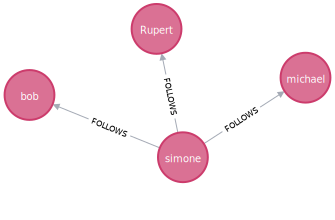
\includegraphics[width=0.8\textwidth]{usersgraph}
	\caption{Users who like Fish and their cities.}\label{fig:usersgraph}
\end{figure}

\figref{fig:usersfollowed} shows the users followed by the current user (named
``simone'').

\begin{figure}[htb]%TODO
	\centering
	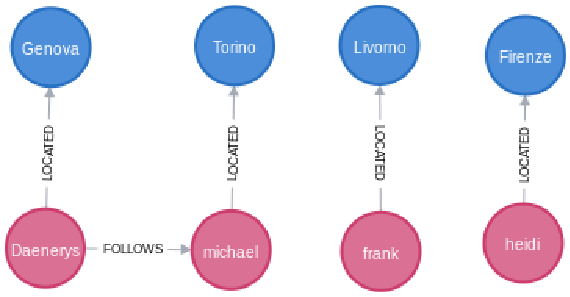
\includegraphics[width=0.8\textwidth]{usersfollowed}
	\caption{Users followed by simone.}\label{fig:usersfollowed}
\end{figure}

So, as you can see from the table in \figref{fig:tableuserform}, the application
returns the correct result as it shows ``frank'' and ``heidi'' users who are the
users who like the Fish cuisine and who live within a radius of 80 kilometers
from Pisa. Note that in the table, as expected, they are sorted by distance from
Pisa.

\begin{figure}[htb]
	\centering
	\includegraphics[width=1\textwidth]{tableuserform}
	\caption{Recommended users by the application.}\label{fig:tableuserform}
\end{figure}

\section{Restaurant Recommendations}

We have tested the recommendation on restaurants, here we are providing an
example of the correctness of our results.

Let's suppose to have the situation shown in~\figref{fig:recommendres1}, looking
at the user ``carol'' and his followers/followed users.

\begin{figure}[htb]
	\centering
	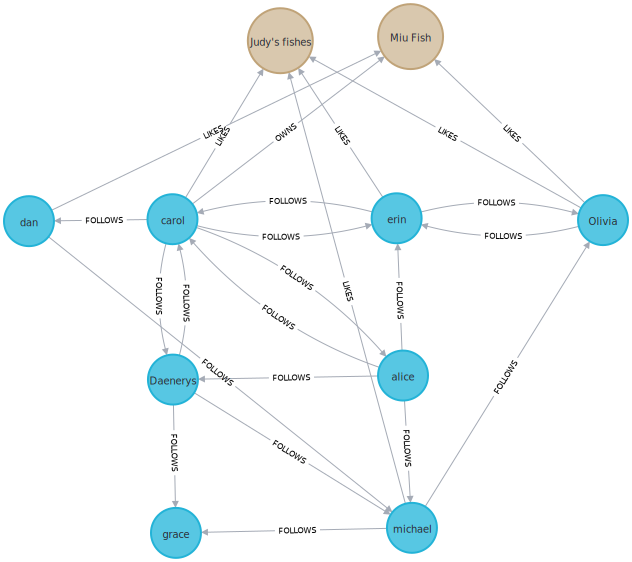
\includegraphics[width=1\textwidth]{test_recommend_rest1}
	\caption{Followers of carol and users followed by carol.}\label{fig:recommendres1}
\end{figure}

Now, suppose that carol want to find a restaurant that \code{SERVES} Pizza with
a price of \code{Luxury} or lower, at most 80 km distant from Livorno. She would
fill the form like in~\figreg{resrecform}.

\begin{figure}[H]
	\centering
	\includegraphics[width=1\textwidth]{test_recommend_filter}
	\caption{Restaurant Recommendations Form.}\label{fig:resrecform}
\end{figure}

In the system we have the Restaurants shown in~\figref{fig:recommendres2} which
serves Pizza.

\begin{figure}[htb]
	\centering
	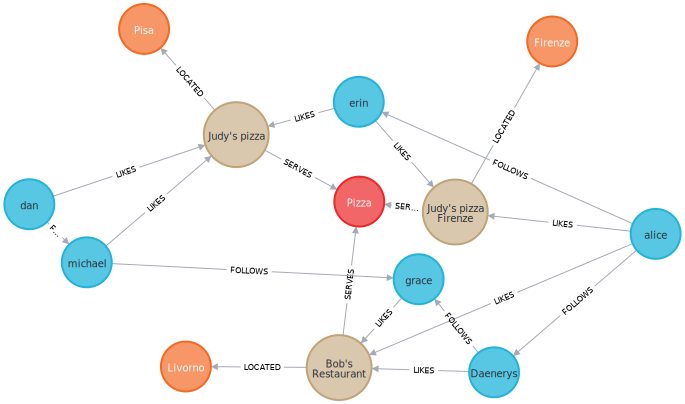
\includegraphics[width=1\textwidth]{test_recommend_rest2}
	\caption{Restuarants which serves Pizza.}\label{fig:recommendres2}
\end{figure}

Now the system will suggest to carol the restaurants which serves pizza ordered
by the number of likes of friends and friends of friends and excluding the
restaurants she already likes or owns.

The result provided by the application is shown in~\figref{fig:recresult}.

\begin{figure}[H]
	\centering
	\includegraphics[width=1\textwidth]{test_recommend_result}
	\caption{Restaurant Recommendations Form.}\label{fig:recresult}
\end{figure}

We can then check in the database that result is correct, in fact looking at the
database we have the situation shown in~\figref{fig:recommendres3}.

In the figure are shown only the relationships from friends or friends of
friends of carol with the restaurants which serves pizza. Counting the
\code{LIKES} relationship we can see that effectively Bob's Restaurant and
Judy's Pizza have 3 likes each other, instead Judy's Pizza Florence has only two
likes, thus is shown after.

\begin{figure}[htb]
	\centering
	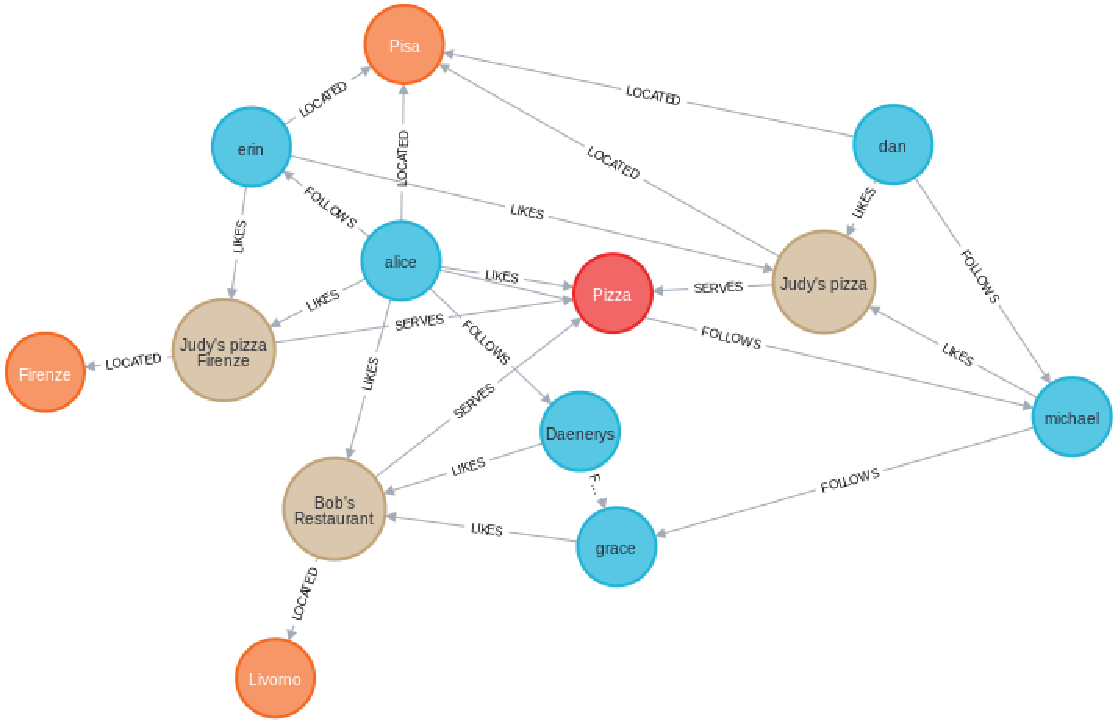
\includegraphics[width=1\textwidth]{test_recommend_rest3}
	\caption{Graph snapshot for restaurant recommendations.}\label{fig:recommendres3}
\end{figure}

Here we can see the results in json:

\begin{verbatim}
    [
  {
    "r": {
"identity": 35,
"labels": [
        "Restaurant"
      ],
"properties": {
"name": "Bob's Restaurant",
"description": "Pizza <3",
"price": "MIDDLE"
      }
    },
    "likes": 3
  },
  {
    "r": {
"identity": 48,
"labels": [
        "Restaurant"
      ],
"properties": {
"name": "Judy's pizza",
"description": "The best pizzas of the world!",
"price": "HIGH"
      }
    },
    "likes": 3
  },
  {
    "r": {
"identity": 49,
"labels": [
        "Restaurant"
      ],
"properties": {
"name": "Judy's pizza Firenze",
"description": "The best pizzas of the world!",
"price": "HIGH"
      }
    },
    "likes": 2
  }
]
\end{verbatim}
